% vim: set textwidth=78 autoindent:

\subsection{Gradnetz Generator Plugin}

% when the revision of a section has been finalized, 
% comment out the following line:
% \updatedisclaimer

Das Plugin \toolbtntwo{grid_maker}{Gradnetz Generator} erlaubt es, f�r
einen ausgew�hlten Kartenausschnitt ein regelm��siges Koordinatengitter aus
Punkten, Linien oder Polygonen zu erstellen. S�mtliche Einheiten m�ssen dabei
in Dezimalgrad eingegben werden. Bei der Ausgabedatei handelt es sich um
einen Shapefile, der 'On-The-Fly' (OTF) passend zu anderen Daten projiziert
werden kann.

\begin{figure}[ht]
\begin{center}
  \caption{Dialog Geographisches Netz Plugin \nixcaption}\label{fig:graticule}\smallskip
  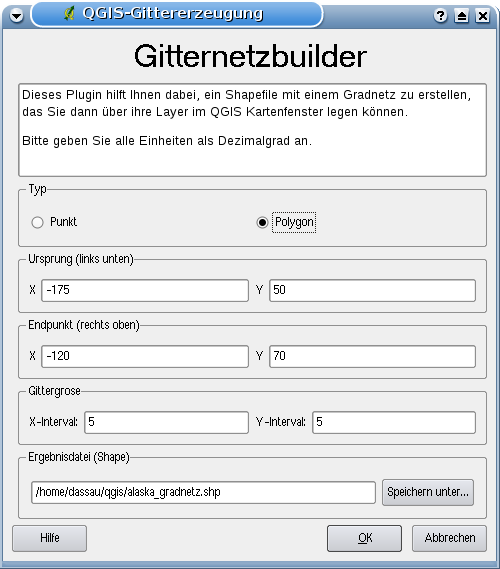
\includegraphics[clip=true, width=10cm]{grid_maker_dialog}
\end{center}
\end{figure}

Hier ein Beispiel f�r die Erstellung eines Gitternetzes:

\begin{enumerate}
\item Stellen Sie sicher, dass das Plugin im Plugin Manager geladen ist (vgl.
Kapitel~\ref{sec:load_core_plugin}).
\item Klicken Sie auf das
\toolbtntwo{grid_maker}{Koordinatenlinien-Generator} Icon in der Werkzeugleiste.
\item W�hlen Sie aus, ob das Gitter aus Punkten, Linien oder Polygonen
bestehen soll.
\item Geben Sie die Breiten- und L�ngengrade f�r die obere linke und rechte
Ecke des Gitters ein.
\item Geben Sie den Abstand an, der bei der Erstellung des Gitters verwendet
werden soll.
Sie k�nnen dabei unterschiedliche X und Y Werte verwenden (L�ngengrad,
Breitengrad).
\item Geben Sie an, wo und unter welchem Namen die Shape-Datei erstellt
werden soll.
\item Klicken Sie dann auf \button{OK} um das Gitternetz zu erstellen und
f�gen Sie dieses abschlie�end dem Kartenausschnitt hinzu.
\end{enumerate}



